\chapter{Syntax Analysis}\label{sec:syntaxAnalysis}
Syntax analysis is the first phase in compiling a language.
In this phase it is checked whether the input adheres to the rules of the language.
These rules are defined in a languages' \acrshort{cfg}.
The \acrshort{cfg} of \gls{gamble} is further described in \myref{sec:cfg}.\todo{Behøver det her nævnes igen ? Ja nej ? - Søren}
This analysis can be split up further into sub phases, lexical analysis and parsing, these are described in this chapter.
A diagram of the part of the compiler responsible for the syntax analysis is shown is in \myref{fig:flowSyntax}.
\vspace{10pt}
\begin{figure}[h]
    \centering
    \begin{tikzpicture}[node distance = 3cm, auto]
        \node (start) [lille] {Source code};
        \node (scanner) [lille, right=0.7cm of start] {Scanner};
        \node (parser) [lille, right=0.7cm of scanner] {Parser};
        \node (pt) [lille, right=0.7cm of parser] {Parse--Tree};
        \node (ast) [lille, right=0.7cm of pt] {Abstract Syntax Tree};
        \node (error) [cloud, above=1cm of parser] {Error report};

        \draw [arrow] (start) -- (scanner);
        \draw [arrow] (scanner) -- (parser);
        \draw [arrow] (parser) -- (pt);
        \draw [arrow] (pt) -- (ast);
        \draw [arrow,dashed] (parser) -- (error);

    \end{tikzpicture}
    \caption{Diagram showing the modules of the syntax analysis. } 
    \label{fig:flowSyntax}
\end{figure}
\vspace{-20pt}

\section{Design}
%Design
\subsection{Scanner}
The first stage of syntax analysis is the scanner, also called the lexer which handles the lexical analysis.
The primary function of a scanner is to transform a sequence of characters into a sequence of tokens.
The scanner makes sure that the source code adheres to the grammar rules provided by the CFG.
An example of this, would be that you could use the notation .1 or 0.1 for a decimal number, both being turned into valid tokens by the scanner.
The scanner provided by ANTLR groups related tokens into token types such as INT, ID and FLOAT.
In ANTLR a token contains at least two pieces of information, the token type and the matched text for the token.

Some examples of our lexical rules for \gls{gamble} can be seen on \myref{lst:token}.
The definition of an integer number on line 3 states that an integer is either a zero or an optional negative sign followed by a single digit from one to nine followed by zero or more numbers from zero to nine.
It is necessary to clearly define tokens for the lexer to read in order to read source code correctly. \citep{Crafting_book}

\begin{lstlisting}[caption=Example of our lexer rules for ANTLR4,frame=tlrb,label={lst:token}]
// Integers
INT: 'int' | 'int16' | 'int32' | 'int64' ; // Integers
INTNUM: '0' | SIGN? [1-9][0-9]* ;

// Matrices and vectors
MATRIX: 'matrix' ;
ROWVECTOR: 'rowvector' | 'rvec' ;
COLVECTOR: 'colvector' | 'cvec' ;  

// Whitespace and comments
WS: [ \t ]+ -> skip;
NL: [ \r \n | \n ] -> skip;

COMMENT
    :   '/*' .*? '*/' -> skip
    ;

LINE_COMMENT
    :   '//' ~[\r\n]* -> skip
    ;
\end{lstlisting}
\subsection*{Parser}\label{subsec:parser}
The parser is based on the \acrfull{cfg} of \gls{gamble} written in \acrfull{ebnf}, whose alphabet consists of tokens produced by the scannar.
The parser reads tokens and groups them into phrases according to the \acrshort{cfg}.
The parser verifies that the syntax is correct and upholds to the \acrshort{cfg}, and if a syntax error is found it provides a corresponding error message. \citep{Crafting_book}
By using a parser generator like \acrshort{antlr} or SableCC, handling of syntactic errors and repairs can be done automatically.
A parser can also be written manually but doing so can result in syntactic errors that is hard to locate or solve.
Writing a parser by hand can also take a lot of time, and it can be difficult to go back and change or add new productions to the syntax, which is something the project group will want to do due to the iterative development.
There are many parser generators which can be used like: SableCC, JavaCC, JFlex and many others, but we have chosen to use \acrshort{antlr}.
\acrshort{antlr} has been chosen due to their special use of the ALL(*) grammar, which poses many opportunities for the grammar, and also makes the \acrshort{cfg} easier to write.
\acrshort{antlr} generates a parser which produces a parse tree that contains information about how the parser have grouped the tokens into more abstract language definitions, such as expressions and statements.

There are different kind of parsers, most common are bottom-up and top-down parsers.
\acrshort{antlr} makes a top-down parser, more specific a recursive descent parser.
A recursive descent parser is a subtype of top-down parser build from a set of mutually recursive procedures where each such procedure implements one of the productions of the grammar.
The structure of the resulting program closely mirrors the grammar it recognizes. \citep{Recursive_programming}
Recursive-descent parsers are a collection of recursive methods, one per rule of the \acrshort{cfg}.
Such a method for an assignment rule may look as shown in \myref{lst:rdpmethod}, where the rule is \texttt{assignment : ID = expr ;}.
So the method expects an ID to be the first token from the tokenstream, then an assignment operator followed by an expression and a semicolon.
Here the expression is a rule itself, and is therefore called on the expected expression.
An error should be returned if anything is not what was expected.
\begin{lstlisting}[caption=Example a recursive descent parser method,frame=tlrb,label={lst:rdpmethod}]
// assign : ID ``='' expr ``;'' ;
void assign() { // method generated from rule assign
match(ID); // compare ID to current input symbol then consume
match('=');
expr(); // match an expression by calling expr()
match(';');
}
\end{lstlisting}

%The second stage of the parser is the actual parser.
%The parser is fed a stream of tokens to recognise a sentence structure and in turn outputs the structure to a parse tree.
%The parse tree records how the parser recognises the structure of the input and its components.
%The parse tree that \acrshort{antlr} provides contains information about how the parser have grouped the tokens into more abstract languange definitions such as expressions and statements.
%Where previous versions of \acrshort{antlr} have also implemented the AST, it is not contained in \acrshort{antlr} V4 instead the parse tree provided by \acrshort{antlr} have been used to generate an AST this is discussed in \myref{sec:AST}.
%This tree is a trimmed version of the parse tree, where the less informative data have been removed, this makes it easier to read, and thus easier to use throughout development of the rest of the compiler.

%2nd stage is the actual parser, feeds of tokens to recognize sentence structure
%Parse tree records how the parser recognized structure of input and its component phrases
%Trees provide an easy to walk data structure that will be helpful for the rest of the compiler
%2.2 Implementing Parser - Recursive descent
%Recursive-descent parsers are really just a collection of recursive methods, one per rule.
%Such a rule may look similar to this
%// assign : ID ``='' expr ``;'' ;
%void assign() { // method generated from rule assign
%match(ID); // compare ID to current input symbol then consume
%match('=');
%expr(); // match an expression by calling expr()
%match(';');
%}
%Descent refers to the fact we start from the root and go down to the leaves(tokens)
%Reursive descent is just one form of top-down parsers.					NOTE topdown/bottom up parsing
%The call graph traaced out by invoking methods, mirrors the interior parse tree nodes
%To Build a parse tree manually one would insert ``add new subroot note' operations at the start of each rule, and a ``add new leaf node'' operation to match()
%The assign method checks if all necessary tokens are present and in the right order. When the parser enters assign it doesnt have to choose between more than one alternative. An alternative is one of the choices on the right side of a rule def. A parsing method for such rule would be a switch which looks for what token is present.
% This is called a parising decision or prediction by examining next token
%This is where lookahead comes into play , the lookahead token is the next input token, this can be any token the parser "sniffs" before consuming
%This is one of the places where \acrshort{antlr} is an especially handy tool to use, because \acrshort{antlr} allows for more lookahead than other parser generators.
%Most parsers use a lookahead of one which LL(1) or LR(1), \acrshort{antlr} tones the lookahead up and down depending on what token stream it is trying to decode, as such the \acrshort{antlr} has a lookahead of LL(*)
%\acrshort{antlr} Solves simple ambiguity simply by using the first mentioned rule.
%AST only useful, Parse all artifacts(space, brackets and so on)


\subsection*{Abstract Syntax Tree}
\todo{to be written}
\subsubsection*{Traversal of Trees}
In the previous section an \acrshort{ast} which contains information from the source code was presented; to get the information from the trees, a tree traversal is needed.
For this task different approaches can be taken, one way is to implement a design pattern called the visitor pattern.
Alternatively one can implement the composite pattern or choose to implement no pattern at all, but simply create a case analysis for each object.
The use of a design pattern is not a requirement for the creation of a compiler.

Design patterns provide a general reusable solution for a software problem, each pattern providing its own benefits.
Using a pattern is not just copy and pasting other's code, but it simply states how to solve the problem at hand using different software structures.\todo{Copy pasting code? Hænger det sammen med design patterns? - Corlin}
In OOP, patterns are often described from a UML diagrams, showing the class and interface structure, and which methods these classes must implement. 

The two aforementioned patterns are classified under two different branches of patterns.
The composite pattern is a structural pattern where the visitor pattern is a behavioural one.
A structural pattern provides a way of defining the relations between objects, the composite pattern is used to create a hierarchical recursive tree structure of related objects that may be accessed in a standardised manner.
A behavioural pattern is instead used to define how the objects communicate, the visitor pattern is used to separate a set of structured classes from any functionality that should be performed upon them.\citep{GOF}
For the compiler the visitor pattern have been implemented for the traversal of trees as such the pattern is described further in the following section. 

\subsubsection*{Visitor Pattern}\label{subs:visit}
The visitor pattern is not only used to traverse the parse tree provided by ANTLR, but also the \acrshort{ast} created in the compiler.
The visitor pattern is implemented throughout the compiler, to create the \acrshort{ast} from the parse tree and for traversing the \acrshort{ast}.
As such the visitor pattern defines the structure of the compiler, and thus understanding the benefit from using the pattern is important.
The visitor pattern is described by the Gang of Four, authors of ``Design Patterns: Elements of Reusable Object-Oriented Software'' as:
``a design pattern that separates a set of structured data from the functionality that may be performed upon it.''. \citep{GOF}

In the tree walk for the parse tree, the visitor should convert the parse tree into a \acrshort{ast}.
This entails that each different node in the parse tree must be visited to find the information needed to create the \acrshort{ast}.

Through use of the visitor pattern the functionality is separated from the classes they are performed upon. 
Instead the functionality is on a visitor class implementing the visitor interface, which means different visitors can be made, which all do different computations while traversing the tree.\todo{måske tasks i stedet for computations. MP}
Each class in the tree have an \texttt{accept()} method that allows them to call the visitor in question with itself as an argument.
This allows the ability of adding new operations without changing the original data structure, and also without changing other visitors.
This also serves well when using a iterative development method.
Another benefit is that a single visitor object is used to visit all the classes in the tree.
This visitor can therefore maintain a state between calls to individual data objects, which can be used to save information in an outer scope from the different visit calls.
\myref{image:visitor} shows an UML diagram of the visitor pattern.
This diagram is from a C\# representation, and while the idea is the same the exact implementation is not identical to the one used in the compiler for \gls{gamble}.
Take note of the classes ``ConcreteElement'' and ``ConcreteVisitor''.
The ``ConcreteElement'' represents the different kinds of nodes in a given tree.
The ``ConcreteVisitor'' represents the different kind of visitors implemented.
A visitor will make sure that the children of the node is traversed in the correct way, and will at the same time also do other computations, e.g. pretty printing or checking the source code for errors.\todo{Skal vi komme med andre eksempler her ? Såsom, type checking or code generating?}
A visitor must implement a method to visit every single ``ConcreteElement'' which exist in the tree.
As can be seen on \myref{image:visitor} ``ConcreteVisitorA'' and ``ConcreteVisitorB'', both implement a visit method for the ``ConcreteElements'' A and B.
In the next section, the implementation of creating the \acrshort{ast} from the parse tree using the visitor pattern will be presented.

\begin{figure}[!ht]
\centering
 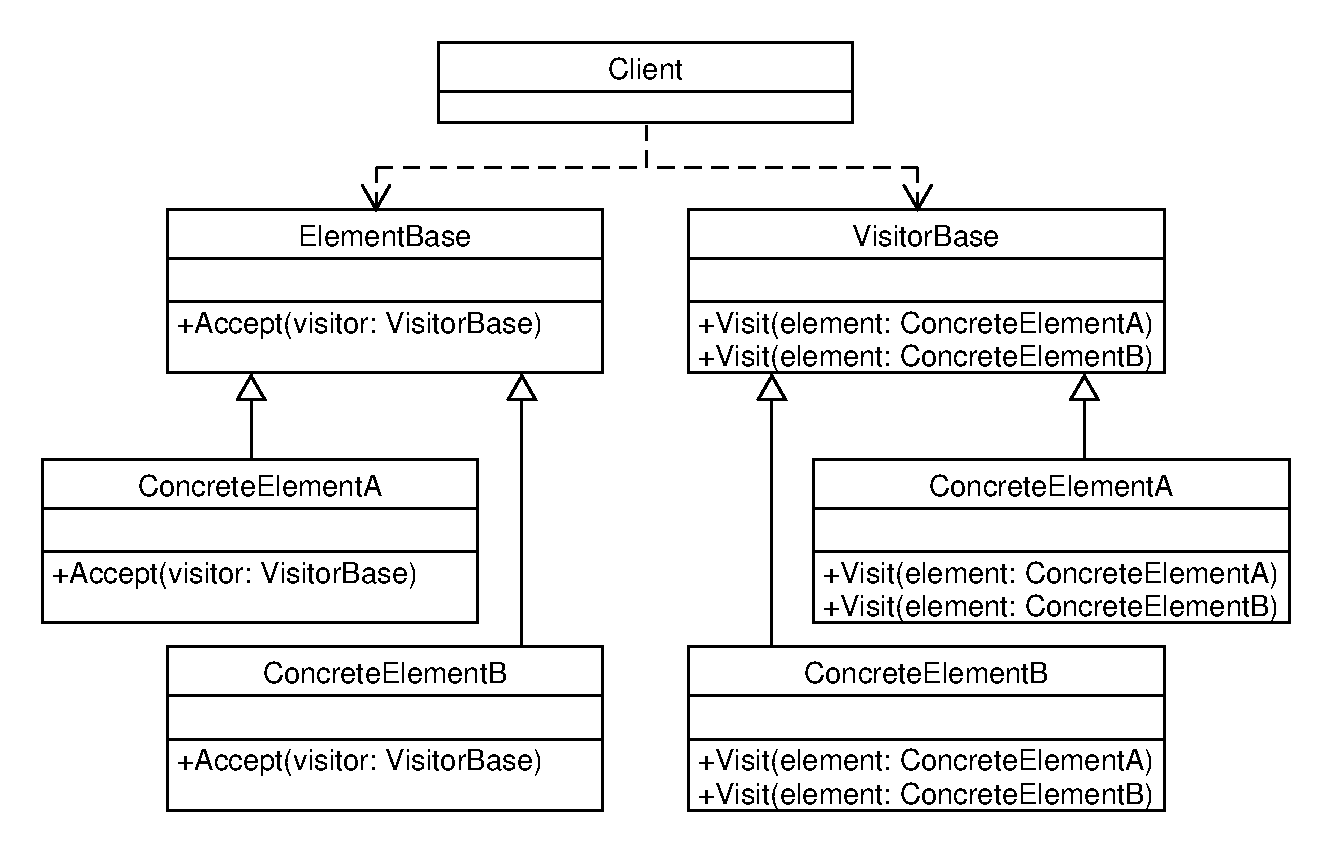
\includegraphics[width=1\textwidth]{figures/ClassDiagrams/VisitorPattern.pdf} % trim=4.85cm 15cm 0.85cm 1cm
\caption{An UML diagram for the implementation of the visitor pattern.}\label{image:visitor}
\vspace{-15pt}
\end{figure}
\todo[inline]{har vi selv lavet figuren? MP - Ja den har jeg lavet :) men der skal nok en kilde på så man kan se hvor vi har det fra, Marc found it. - Søren}

\subsection{Creating the \acrshort{ast}}\label{CreatingAst}

The goal for the \acrshort{ast} is to decrease the information in the tree.
The hidden information is then contained in fields created for the respective classes.\todo{Kan ikke finde ud af om det er lidt for groft at sige hidden information? - Søren}
Rather than having the information as fields one could also choose to have this information as children of the nodes.
This would mean that to find the information one would have to run through the children of the nodes without knowing what children it has.
The method chosen for this compiler has the information kept on the fields of a node rather than as children.
The advantage being that the information is kept together without clustering the tree and increasing the readability of the compiler.
All the nodes of the \acrshort{ast} have been designed with this in mind.
For example on figure \myref{image:ASTDecl} a class structure can be seen, which consists of all the classes needed to express a declaration from the \acrshort{cfg} on the tree.
A declaration could be \texttt{int a = 5;}.

\begin{figure}[!ht]
\centering
 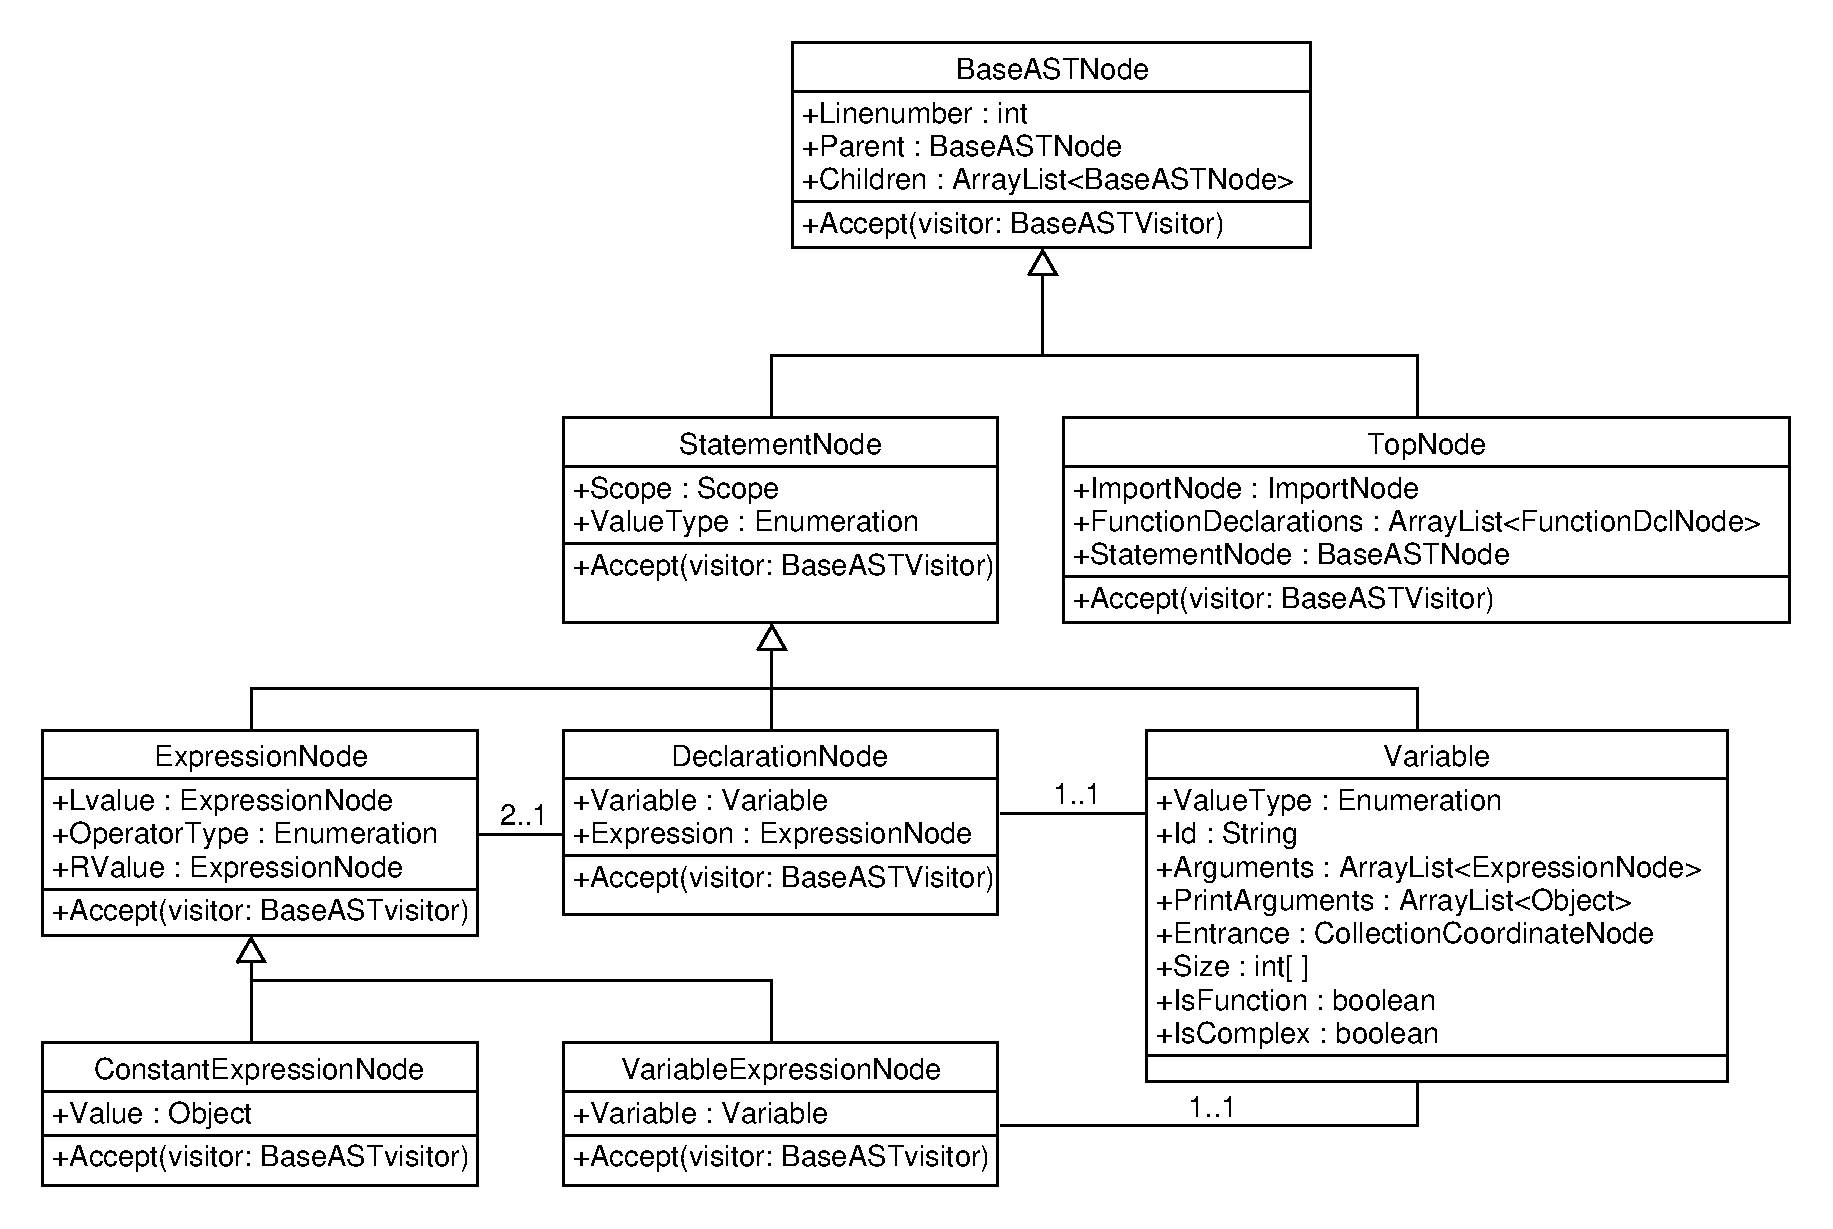
\includegraphics[width=1\textwidth]{figures/ClassDiagrams/ASTDeclarationNodeMoreInfo.pdf} % trim=4.85cm 15cm 0.85cm 1cm
\caption{A UML class diagram of the classes used for a DeclarationNode on the \acrshort{ast}.}\label{image:ASTDecl}
\vspace{-15pt}
\end{figure}

The \texttt{Variable} class contains a lot of different information which is used depending on which class a given instance of \texttt{Variable} is connected to.
If \texttt{Variable} is connected to a \texttt{VariableExpressionNode}, the only fields used on the variable class is ValueType and Id, while the booleans IsFunction and IsComplex are set to false.
In the example \texttt{int a = 5;} the tree structure looks like the AST on \myref{image:AST}.
When the right hand side of an assignment or declaration is a function, an example being \texttt{int a = foo(5);} the fields used on \texttt{Variable} differs from the previous example and instead becomes Id, ValueType, arguments, and the boolean IsFunction is now set to true.
The print argument field is used when a function call to \texttt{print()} is made. 
Entrance, Size and IsComplex are used when dealing with the complex data types, vectors and matrices.
\texttt{TopNode} sets the structure of a \gls{gamble} program as described in \myref{subsec:Struc}.
The full class diagram can be seen in \myref{ASTNodes}.

The classes have made it more intuitive to perform a traversal of the tree based upon the names of the fields on the classes.
E.g. the \texttt{ForLoopNode} has fields named \texttt{Body}, \texttt{Initialize}, \texttt{Update}, and \texttt{Conditional}, these names have meaning instead of just being children on the node which will increases the readability of the compiler.

The syntax analysis phase returns the \acrshort{ast} so it can be used in the next phase, the contextual analysis. 
The design of the phase and the call from main can be seen on \myref{fig:syntaxphase}.\todo{call from main kunne thomas ikke lide. MP - Tror det var fordi han ikke havde set figuren i compiler overview som viser alle kaldene fra main, og dermed var han forvirret over det ? Men ved det self ikke, synes bare ikke det gør noget når man også har set den figur. - Søren}
As can be seen the \texttt{GenerateASTVisitor} makes use of the classes shown in \myref{ASTNodes}.

\begin{figure}[ht]
  \centering
    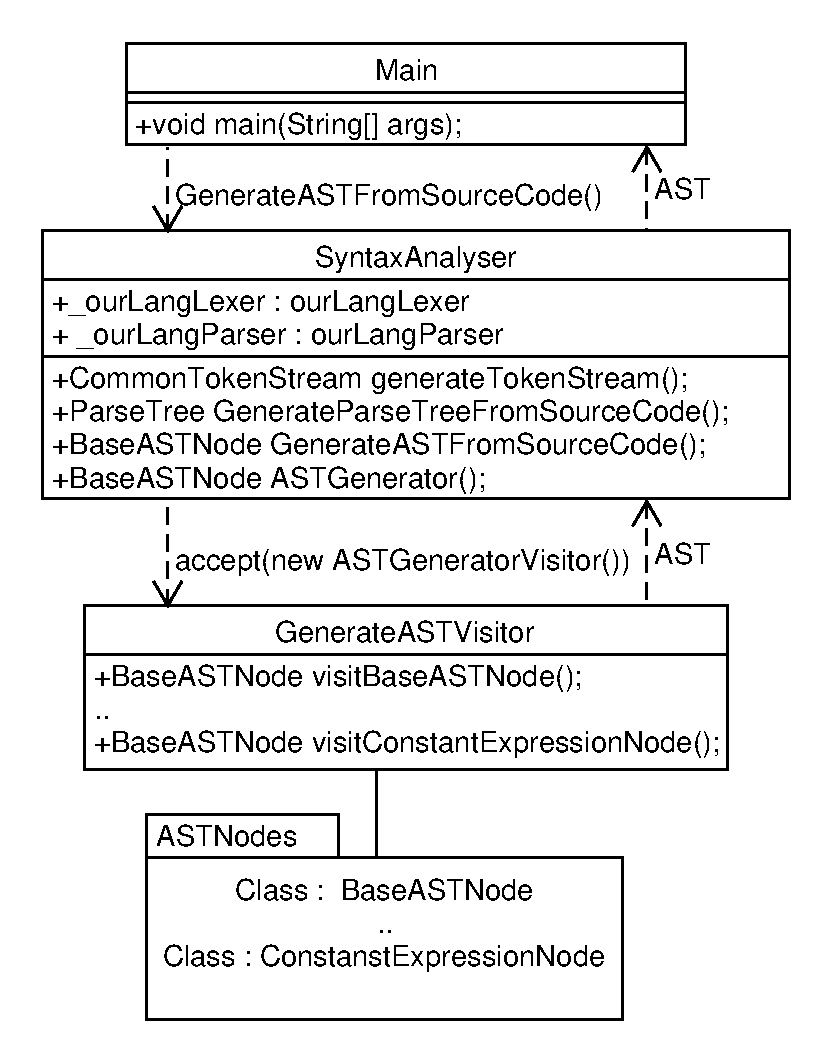
\includegraphics[width=0.48\textwidth]{figures/ClassDiagrams/SyntaxAnalyser.pdf}
  \caption{The function calls and returns in the Syntax Analysis phase.}
  \label{fig:syntaxphase}\todo{Skal vi vise at generateParseTreeFromSourceCode kaldes af ASTFromSourceCode eller noget ? - Søren}
\end{figure}

%Implementation
\section{Implementation}\label{sec:ANTLR}
The syntax analysis is implemented through the tool \acrfull{antlr}, this tool provides some advantages over other available tools.
\acrshort{antlr} is based upon a parser technique called LL(*).
LL(*) uses an algorithm to have a varying lookahead when needed.
The LL(*) parsers, which is a parser that upholds an LL(*) grammar, does not allow a bigger class of \acrshort{cfg}s than other parsers like LL(k), but can change the number of tokens needed as lookahead dynamically. 
In the most recent version of \acrshort{antlr} as time of this publication, \acrshort{antlr}4, the underlying algorithm have been extended to a parser technique called Adaptive LL(*) (ALL(*)).
An important feature of ALL(*) is it moves grammar analysis to parse time and thereby lets the algorithm accept any non-left-recursive productions.
On top of that \acrshort{antlr} allows simple left recursions by rewriting them before parse time.

The \acrshort{antlr} approach accepts a broader class of grammars than most other parsing methods, one way this is done is to rule out ambiguity by using a rule of precedence.
If a grammar is ambiguous the ALL(*) approach will take the first available rule in the \acrshort{cfg} and apply it.
This allows for more opportunities in the \acrshort{cfg} and while most grammars could be rewritten to be unambiguous without applying the precedence rule.
The idea with the ALL(*) algorithm is that the grammar is analysed at parse-time, and requires no static analysis of the grammar. 
This means that the undecidability of static LL(*) grammar analysis is avoided and instead it is possible to make correct parsers for any non-left-recursive \acrshort{cfg}.
This allows \acrshort{antlr} access to input sequences while reading through the grammar, meaning not all possible inputs must be considered.
Due to this dynamic analysis \acrshort{antlr}4 is able to handle some ambiguous constructs and reduce-reduce conflicts.
As mentioned this allows \acrshort{antlr} to take care of left-recursion if such is present in the grammar by rewriting it, as such would be the case in \myref{lst:amb}.

\begin{lstlisting}[caption=An ambiguous rule for expr, which ANTLR handles by applying the first rule of the production if possible,frame=tlrb,label={lst:amb}]
expr : expr '*' expr 	#MulExpression // match expressions with * operator
     | expr '+' expr 	#AddExpression// match expressions with + operator
     | INT 		// matches simple integer
     ;
\end{lstlisting}
\myref{lst:amb} implements \acrshort{antlr}s way of representing operator precedence by simply obeying the first alternative in the rule set, as such the multiplication operator (``*'') will have the higher precedence.
The ALL(*) algorithm also means that one can completely disregard lookahead and it will still be able to parse, although one should keep in mind that having more lookahead than necessary will slow down the process of parsing.
The scanner provided by \acrshort{antlr} groups related tokens into token types such as INT, ID and FLOAT.
In \acrshort{antlr} a token contains at least two pieces of information, the token type and the matched text for the token.
\acrshort{antlr} also implements rule element labels in its \acrfull{cfg} which means one can apply label rules to a construct in a grammar, this allows for conditional steps in the grammar based on the source code being parsed.
The labels on \myref{lst:amb} are \texttt{\#MulExpression} and \texttt{\#AddExpression}.
Furthermore \acrshort{antlr} can set up an interface and base implementation of the visitor pattern for the parse tree on a given grammar by running \acrshort{antlr} with the \texttt{--visitor} flag. \citep{ALLSTAR, LLSTAR, antlr4_Book}

\subsubsection*{Implementation of Creating the \acrshort{ast}}

The class \texttt{VisitorAST} creates the \acrshort{ast} from the parse tree, it traverses the tree using the visitor pattern and on every node sets a field of a class in the \acrshort{ast}. 
Afterwards the node is placed on the tree as a leaf or a field on the node which made the \texttt{visit()} call.

One of these visit methods can be seen on \myref{lst:VisitorASTCode}.

\begin{lstlisting}[caption=The visit method for WhileLoopNode,frame=tlrb,label={lst:VisitorASTCode}]
public BaseASTNode visitWhileLoop(ourLangParser.WhileLoopContext ctx) {
    WhileLoopNode whileLoopNode = new WhileLoopNode(parentStack.peek());
    whileLoopNode.setCondNode(
    	(ConditionalExpressionNode)visit(ctx.conditionalExpression()));
    parentStack.push(whileLoopNode);
    visitChildren(ctx.whileBlock);
    parentStack.pop();
    whileLoopNode.setLineNumber(ctx.start.getLine());
    return whileLoopNode;
}
\end{lstlisting}
A stack called the parentstack is used to keep track of the caller to \texttt{visit()}, in order to keep track of the parents and the children of the tree.
On lines three and four on \myref{lst:VisitorASTCode} a call to visit the \texttt{conditionalexpression} of the whileloop is made, which returns an instance of the class \texttt{ConditionalExpressionNode}.
Afterwards, to set the body of the \texttt{WhileLoopNode}, all the children of the nodes are visited, but first the \texttt{WhileLoopNode} is pushed to the parentstack.
This makes it possible to check which node is the parent of the children being created during the calls to visit.
\acrshort{antlr} uses the implementation where each node has a number of children, and therefore the \texttt{WhileLoopContext} has its children visited rather than specific fields.
While implementing the Visitor pattern for the \acrshort{ast} an interface was made, which contains a visit method for every single class of the \acrshort{ast}.
A baseclass which implements this interface which implements a visit method for all the nodes of the \acrshort{ast} such that the correct fields of the nodes are visited in the intended order.
This means that any visitor class only has to override the visit methods which are of interest for the specific visitor and the ones not overridden will use the baseclass' implementation which simply visits its fields.
An UML diagram for the implementations of the visitor pattern in the compiler and can be seen on \myref{image:Visitors}.
The figure shows how every visitor class inherits from the \texttt{BaseASTVisitor} class.\todo{Overvejer lidt om denne figur skal væk da det jo er design og egentlig bare viser det som figuren i design viser? - Søren}
Now that the Syntax analysis phase is done it is time for the \acrshort{ast} to be send to the contextual analysis phase which the next chapter will cover.

\begin{figure}[!ht]
\centering
 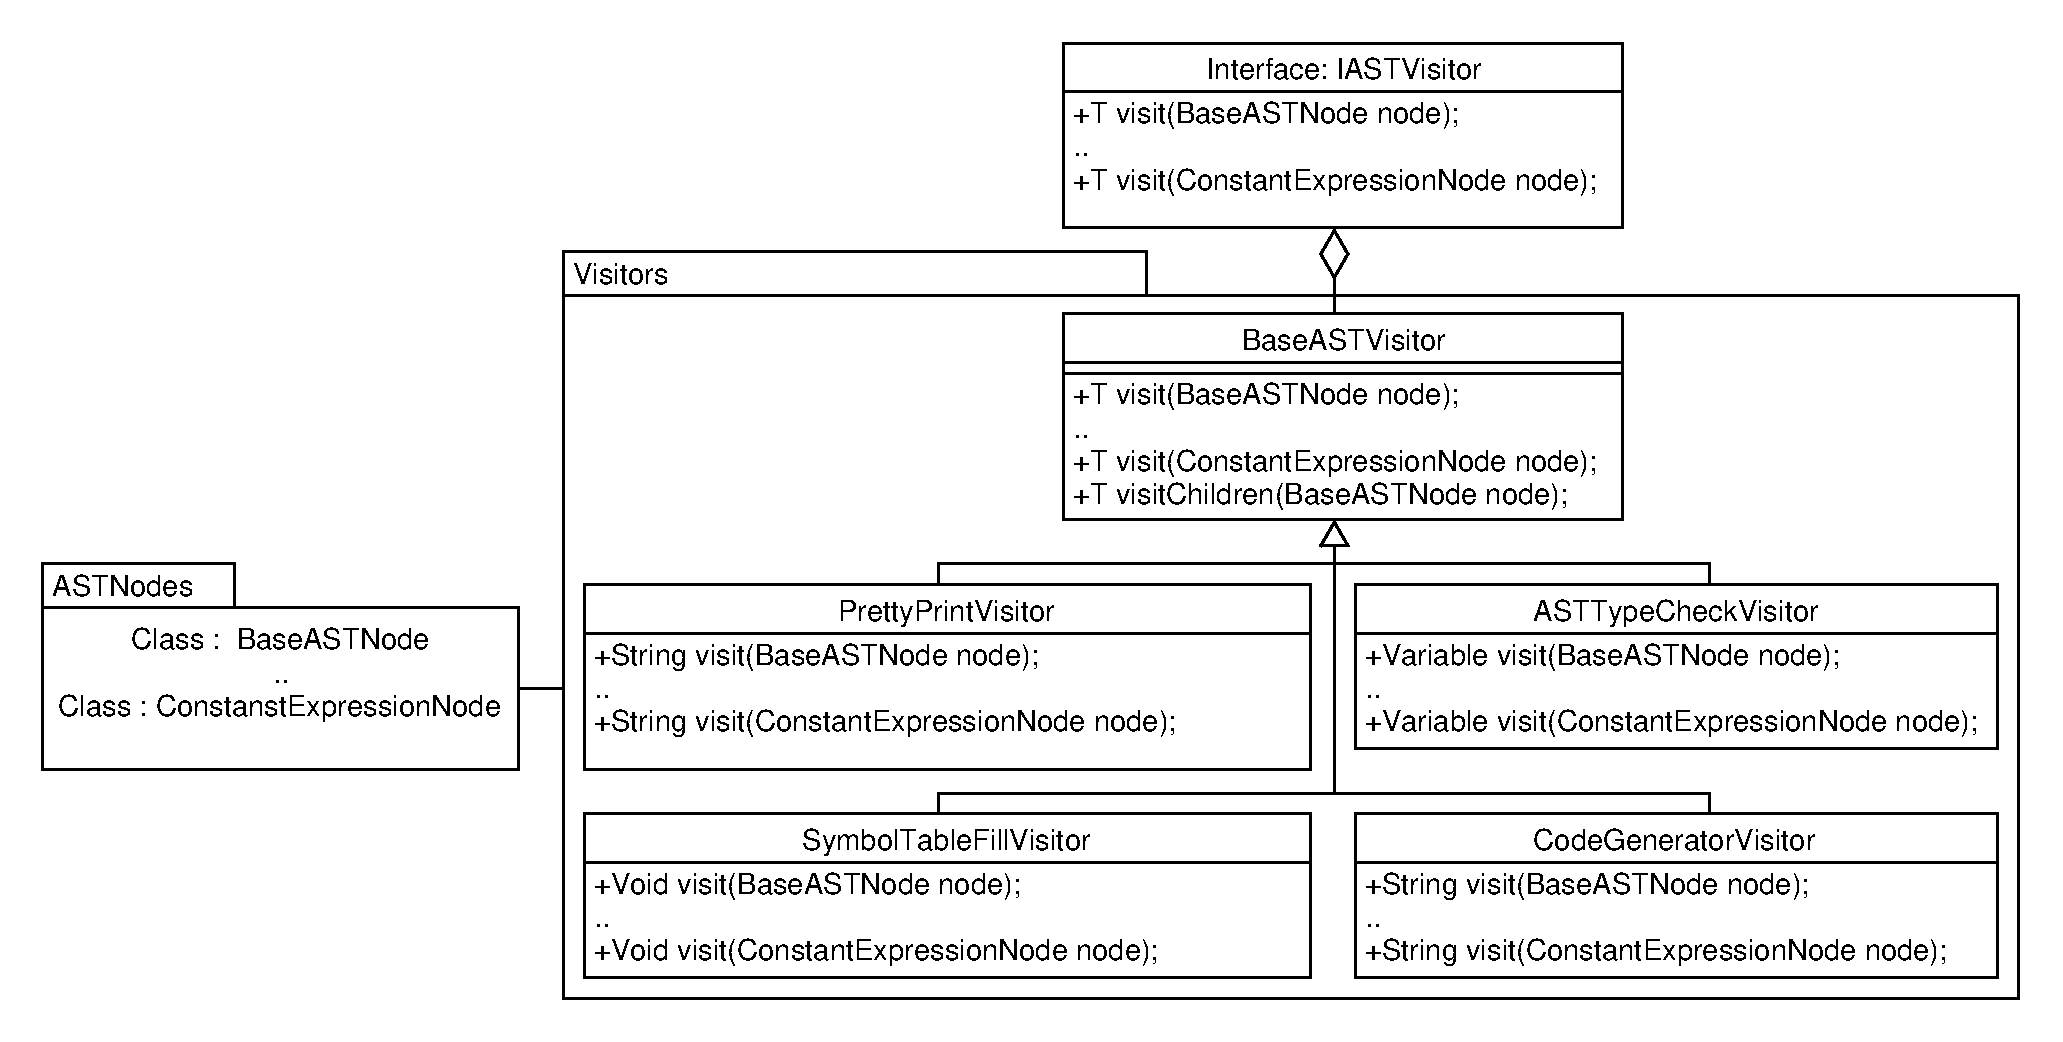
\includegraphics[width=1\textwidth]{figures/ClassDiagrams/Visitors.pdf} % trim=4.85cm 15cm 0.85cm 1cm
\caption{An UML diagram of the visitor patterns implementation in the compiler for traversing the \acrshort{ast}.}\label{image:Visitors}
\vspace{-15pt}
\end{figure} 
